\section*{Aspect Organisationnel}
\myparagraph{Diagramme}
\begin{center}
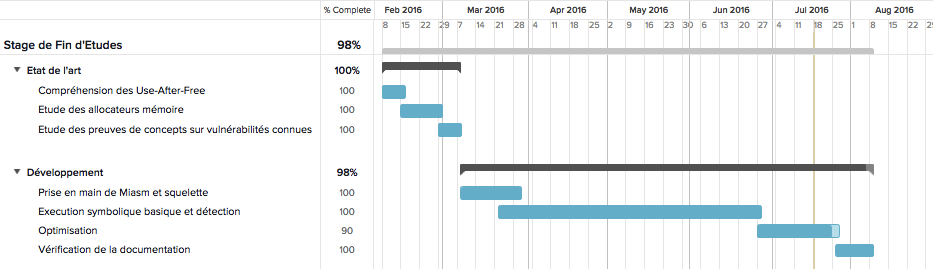
\includegraphics[scale=0.5]{gant.png}\newline
\end{center}

\myparagraph{Organisation et démarrage au sein de l'équipe de test d'intrusion}
Les bureaux de l'équipe étant déjà occupés, les stagiaires étaient disposés dans une salle annexe, tout en restant dans la zone sécurisée propre aux équipes de
la R\&D, du test d'intrusion, et du CESTI (Centre d'Évaluation de la Sécurité des Technologies de l'Information). L'ensemble de l'étage est accessible par des badges, remis lors de la première semaine par la responsable de la
sécurité. Ces badges permettaient d'assurer les mouvements au sein de SOGETI, à la fois pour les ascenseurs, l'accès à la zone sécurisée, ou bien au bureau
de l'équipe. Ce dispositif permet d'assurer l'autonomie complète des stagiaires qui pouvaient circuler librement dans cet espace. En terme de restrictions,
le maitre de stage ou un référent devait être présent durant les horaires de présence du stagiaire, des règles précises de circulation étant en place pour la zone sécurisée.

\subparagraph{}
Même si les maitres de stage n'étaient pas présents dans le même bureau, la discussion était assurée soit par les moyens de communication mis en
place (channel IRC, mail), soit par la proximité des bureaux. Les déjeuners (et autres pauses) se prenaient également avec toute l'équipe, ce qui permettait
d'avoir une certaine proximité avec tous les membres. Les discussions n'étaient pas filtrées et cela rendait possible la compréhension du fonctionnement d'une
ESN et des missions de test d'intrusion en général.

L'équipement de travail a été fourni durant la première journée : ordinateur portable, souris, écran. Le manager de l'équipe et les responsables du matériel
informatique étaient également à l'écoute en cas d'insuffisance technique du matériel mis à disposition.


\myparagraph{Respect et critiques du découpage}
Le planning a été élaboré dans les grands traits lors de la première semaine de stage et a permis de bien structurer
le stage et les durées allouées à chacune des tâches. L'ensemble du découpage a été respecté à la lettre. Les parties
concernant l'état de l'art étaient interrompues en cas d'échéance. En effet, les études étaient déjà assez avancées et le plus
important restait le developpement de l'outil en lui-même.

\myparagraph{Contrôle et réunion d'avancement}
L'avancée du projet a été suivie régulièrement avec un maximum de 2 semaines entre chaque point de contrôle. Durant ces réunions,
les points abordés étaient : les problèmatiques rencontrées, les futures étapes, les dates approximatives de fin de ces étapes.

\subparagraph{}
Le projet était également disponible sur un dépot de versionnement (git) sur l'infrastructure de l'ESEC. Des contrôles pouvaient donc être
fait même en dehors des séances de réunions. Des présentations étaient également effectuées toutes les deux semaines en début de stage, puis plus
espacées, afin de montrer le travail réalisé et prendre l'avis de l'équipe.
